\subsection*{\textbf{Задание 11.6} Работа со списками.}
Создайте два списка из $10$ элементов, а второй из $4$ элементов
по $3$ элемента, и попробуйте все приведенные выше операторы на этих списках.

\begin{figure}[H]
    \renewcommand{\figurename}{Рисунок}
    \centering{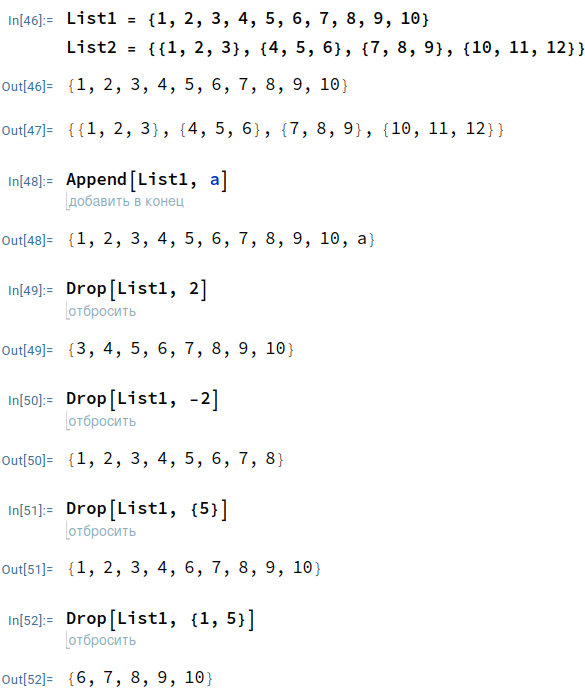
\includegraphics[scale=0.70]{body/img/6_1.png}}
    \label{fig:image_6_1}
\end{figure}

\begin{figure}[H]
    \renewcommand{\figurename}{Рисунок}
    \centering{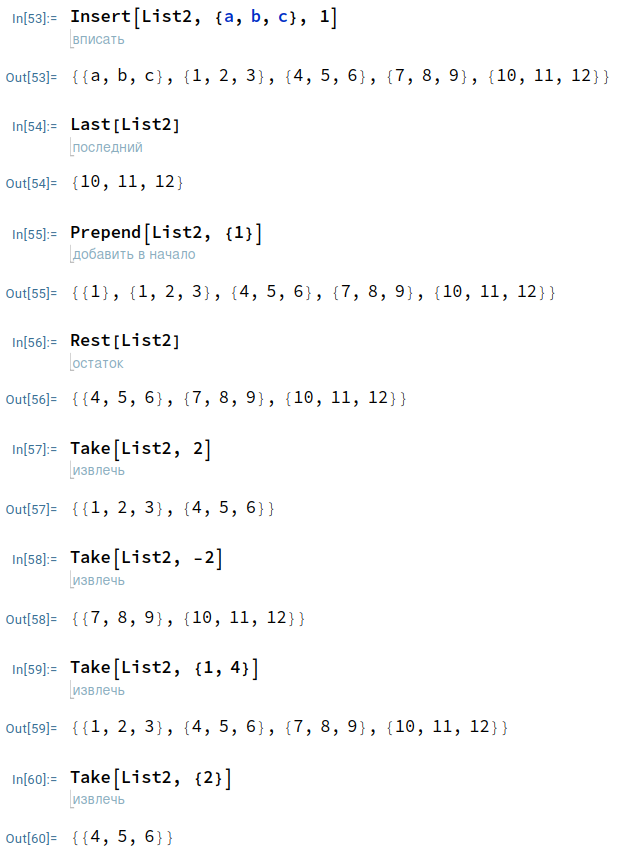
\includegraphics[scale=0.70]{body/img/6_2.png}}
    \label{fig:image_6_2}
\end{figure}

\begin{figure}[H]
    \renewcommand{\figurename}{Рисунок}
    \centering{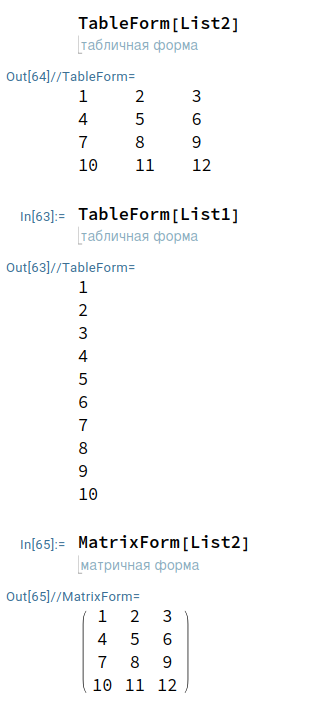
\includegraphics[scale=0.70]{body/img/6_3.png}}
    \label{fig:image_6_3}
\end{figure}